\documentclass{notes}
\usepackage[makeroom]{cancel}

\author{Ritchie Cai, Matthew Mosley \& Corey Higgins}
\title{Inverted Pendulumn Modeling}

\begin{document}
\maketitle 

\section{Description}
Our design project is to simulate and implement a inverted pendulum using 
$\text{Lego Mindstorm EV3}^{\textregistered}$. 

\section{Physical Model}

The rod on top of the cart can only lean forward and backward. 
Base cart also can move only move back and forth. 
When the rod is out of balance and leaning toward one side, the cart will accelerate toward the same
direction to make sure the rod is back to resting position relative to the cart.

\begin{figure}[!h]
  \begin{center}
    \includegraphics[width=2 in]{pics/Full_System_2.eps}
  \end{center}
  \caption{System setup for inverted pendulum}
  \label{fig:full_system}
\end{figure}


\section{Mathematical Model}



\subsection{X-axis}
On the horizontal, x-axis, we have:

\begin{align*}
  % F_x & = F_{cart} + F_{rod} \\
  % F_{cart} & = M\ddot{x}  \\
  % F_{rod}  & = m a_x + m a_{p} \\
  %         & = m \ddot{x} + m (a_{t} + a_{c})
  F_x & = (M+m) \ddot{x} + m (a_{t} + a_{c})
\end{align*}

where $a_t$ and $a_c$ are tangential and centripetal acceleration respectively. 

\begin{figure}[!h]
  \begin{center}
    \begin{minipage}[b]{3.5in}
      \centerline{\mbox{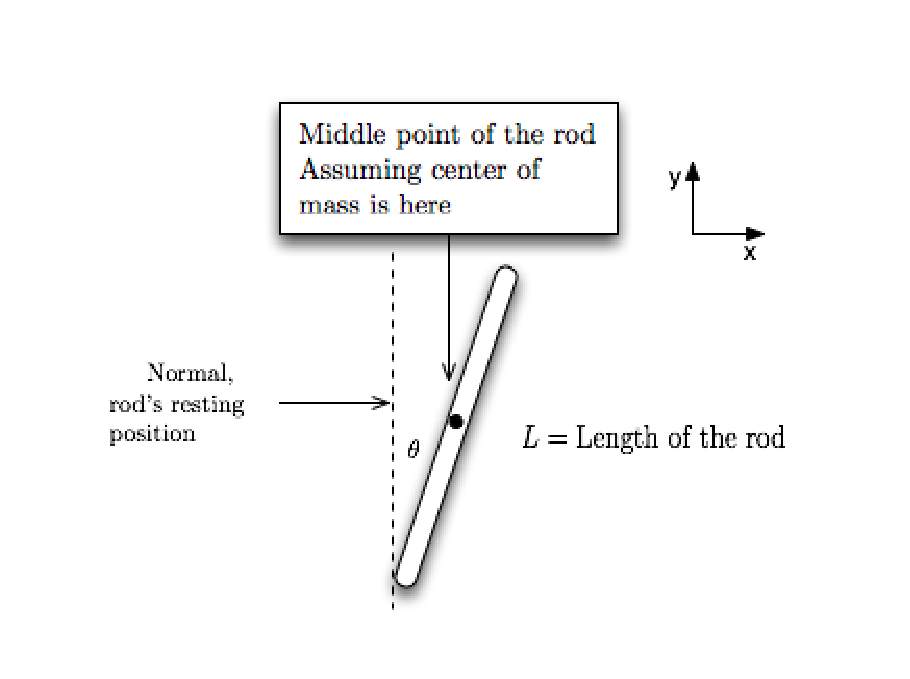
\includegraphics[width=3.5in]{pics/rod.eps}}}
    \end{minipage}
    \begin{minipage}[b]{3.5in}
      \centerline{\mbox{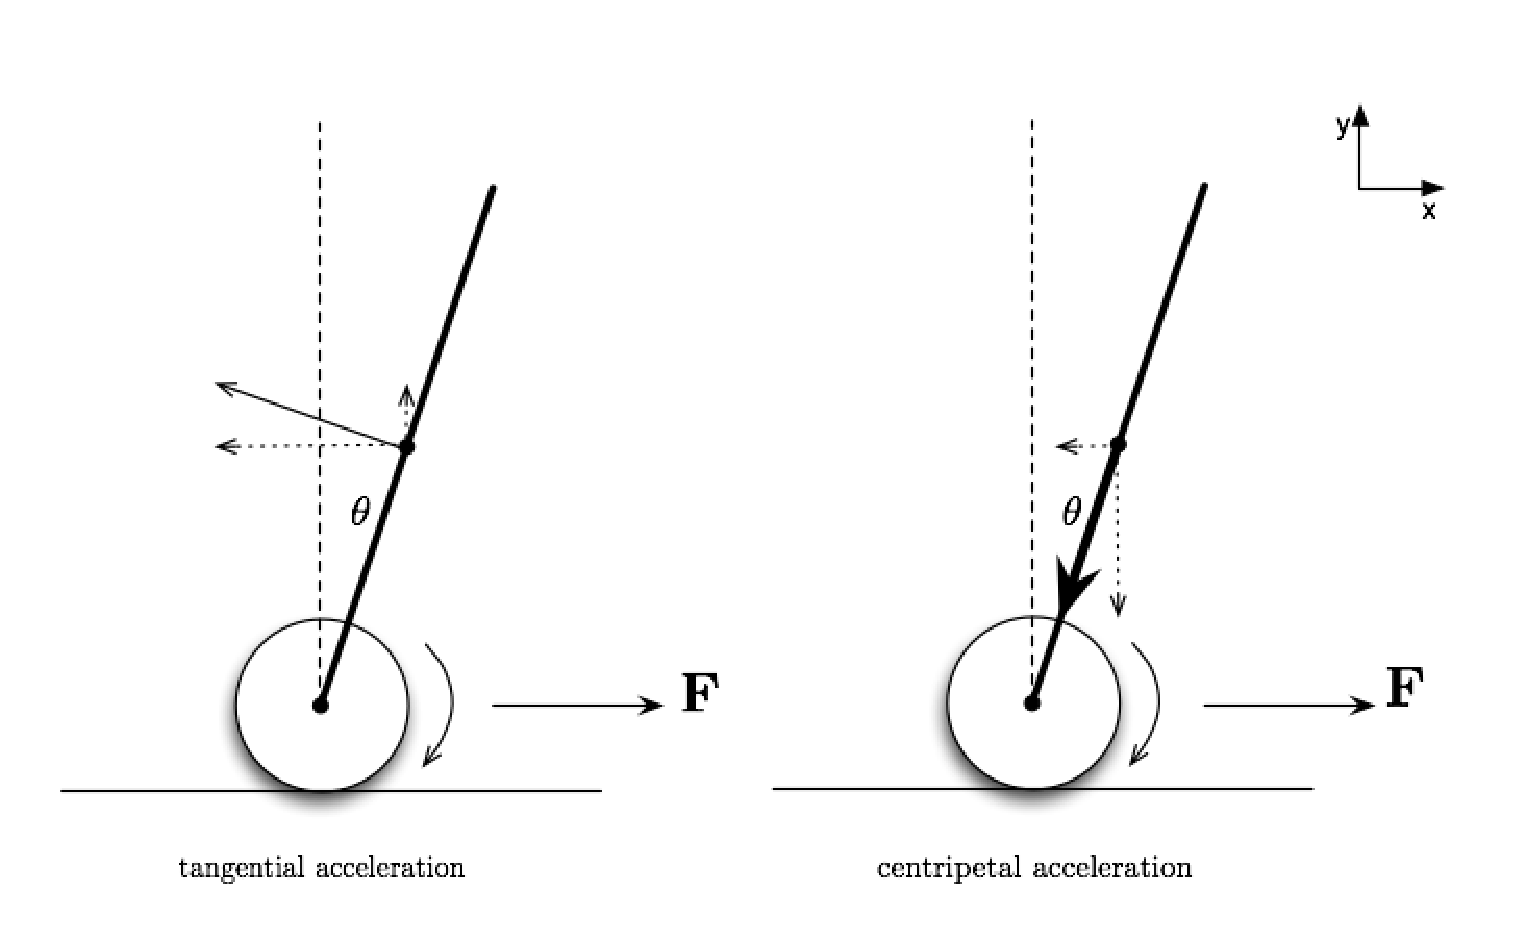
\includegraphics[width=4.5 in]{pics/rod_acc.eps}}}
    \end{minipage}
    
  \end{center}
  \caption{Angular acceleration disection for the rod}
  \label{fig:angular_rod}
\end{figure}

According to figure~\ref{fig:angular_rod}, angular accelerations for the rod on x-axis can be
expressed as:
\begin{align*}
  a_t & = -\dfrac{L}{2} \ddot{\theta} \\
  a_c & = -\dfrac{L}{2} \dot{\theta}^2
\end{align*}

Since we are only interested in the components on the x-axis, we have:

\begin{align*}
  a_t & = -\dfrac{L}{2} \ddot{\theta} \cos \theta \\
  a_c & = -\dfrac{L}{2} \dot{\theta}^2 \sin \theta
\end{align*}

So 

\begin{align}
  F_x & = (M+m) \ddot{x} + m (a_{t} + a_{c})\nonumber\\
         & = (M+m) \ddot{x} -m\dfrac{L}{2} \ddot{\theta} \cos \theta 
                        -m\dfrac{L}{2} \dot{\theta}^2 \sin \theta 
%	      & = (M + m) \ddot{x} - m\dfrac{L}{2} \ddot{\theta} \cos \theta 
%	                     - m \dfrac{L}{2} \dot{\theta}^2 \sin \theta
\end{align}
\FloatBarrier


\subsection{Y-axis}
Using Newton's second law for the vertical motion of the pendulum gives

\begin{align*}
  % F_y & = ma_y - mg \label{eqn:eq1} \\
  F_y & = ma_y - mg \\
      & = m(a_t + a_c) - mg
\end{align*}
where $a_y$, $a_t$ and $a_c$ are acceleration of y-axis, tangential and centripetal of the rotation
respectively. 

Using figure~\ref{fig:angular_rod}, we can express the acceleration on y-axis with:
\begin{align*}
  a_t & = \dfrac{L}{2}\ddot{\theta}\sin\theta \\
  a_c & = -\dfrac{L}{2}\dot{\theta}^2\cos\theta
\end{align*}

So

\begin{align}
  F_y & = m(a_t + a_c) - mg \nonumber\\
      & = m(\dfrac{L}{2}\ddot{\theta}\sin\theta - \dfrac{L}{2}\dot{\theta}^2\cos\theta) - mg
      \nonumber\\ 
      & = m\dfrac{L}{2}\ddot{\theta}\sin\theta - m\dfrac{L}{2}\dot{\theta}^2\cos\theta - mg
       \label{eqn:f_y}
\end{align}

 % Since $ y = \dfrac{L}{2}\cos\theta$,

 % \begin{align}
 %   \dot{y} & = \frac{d(l/2\cos\theta)}{dt} = -\dfrac{L}{2}\ddot{\theta}\sin\theta \nonumber\\
 %   % \frac{dy_G}{dt} & = \frac{d(l/2\cos\theta)}{dt} = -l/2\sin\theta\frac{d\theta}{dt} \nonumber\\
 %   \frac{d^2y_G}{dt^2} & = \frac{d}{dt}\left(-l/2/2 \sin\theta \frac{d\theta}{dt}\right) \nonumber\\
 %   & = -l/2/2\left(\frac{d\sin\theta}{dt}\frac{d\theta}{dt} + \sin\theta\frac{d^2\theta}{dt^2}\right) \nonumber\\
 %   & = -l/2\left( \cos\theta \left(\frac{d\theta}{dt}\right)^2 + \sin\theta\frac{d^2\theta}{dt^2}   \right) \nonumber\\
 %   & = -l/2\cos\theta\left(\frac{d\theta}{dt}\right)^2-l/2\sin\theta\frac{d^2\theta}{dt^2}\label{eqn:eq2}
 % \end{align}
 
 % Using Equation~\ref{eqn:eq2}, Equation~\ref{eqn:eq1} can be written as 
 % \begin{align*}
 %   F_y - mg & = m(-\frac{L}{2}\dot{\theta}^2\cos\theta - \frac{L}{2}\ddot{\theta}\sin\theta )
 % \end{align*}
 
 % Thus, the vertical reaction force, $F_y$, can be written as
 % \begin{align*}
 %   F_y & = mg + m\left(-\frac{L}{2}\dot{\theta}^2\cos\theta - \frac{L}{2}\ddot{\theta}\sin\theta\right)
 % \end{align*}

 \subsection{Angular Momentum}
 
 For any object, the relationship between the moment applied on an object and its angular acceleration is given by the following relationship
 \begin{align}
   I \ddot{\theta} = \sum \overline{M} \label{eqn:torque}
 \end{align}
 
 where $\overline{M}$ is the moment due to a given force and defined as 
 
 \[
 \overline{M} = \vec{F} \times \vec{r}
 \]
 
 where $\vec{F}$ is the force vector, $\vec{r}$ is the position vector of the object with respect to
 the point about which the moments are being summed, and $I$ is the angular momentum of the object.
 For the pendulum, summing the moment around the center of gravity, Equation~\ref{eqn:torque} can be
 written as

 \begin{eqnarray*}
   I\ddot{\theta} & = & F_y\dfrac{L}{2}\sin\theta - F_x\dfrac{L}{2}\cos\theta \\
     & = & \left( m\dfrac{L}{2}\ddot{\theta}\sin\theta - m\dfrac{L}{2}\dot{\theta}^2\cos\theta 
            - mg\right) \dfrac{L}{2}\sin\theta \\
     &   & -\left( (M+m)\ddot{x} - m\dfrac{L}{2}\ddot{\theta}\cos\theta - 
             m\dfrac{L}{2}\dot{\theta}^2\sin\theta \right) \dfrac{L}{2}\cos\theta\\
     & = & m\dfrac{L^2}{4}\ddot{\theta}\sin^2\theta 
           - \cancel{m\dfrac{L^2}{4}\dot{\theta}^2\cos\theta\sin\theta} - \dfrac{L}{2}mg\sin\theta\\
     &   & - (M+m) \dfrac{L}{2} \ddot{x}\cos\theta + m\dfrac{L^2}{4}\ddot{\theta}\cos^2\theta + 
             \cancel{m\dfrac{L^2}{4}\dot{\theta}^2\sin\theta\cos\theta} \\
     & = & m\dfrac{L^2}{4}\ddot{\theta}\cancelto{1}{(\sin^2\theta + \cos^2\theta)}
           - \dfrac{L}{2}mg\sin\theta - (M+m) \dfrac{L}{2}\ddot{x}\cos\theta \\
     & = & m \dfrac{L^2}{4}\ddot{\theta} - \dfrac{L}{2}mg\sin\theta 
           - (M+m) \dfrac{L}{2} \ddot{x}\cos\theta
    %               & = & (mg 
    %                    + m(-l\ddot{\theta}\cos\theta - l\ddot{\theta}\sin\theta)
    %                   )l\sin\theta 
    %                   -m(\ddot{x} 
    %                       - \ddot{\theta}l\sin\theta + \ddot{\theta}l\cos\theta
    %                   )l\cos\theta \\
    % & = & mgl\sin\theta - ml^2\ddot{\theta}\cos\theta\sin\theta- ml^2\ddot{\theta}\sin^2\theta \\
    % &  & - ml\ddot{x}\cos\theta + ml^2\ddot{\theta}\cos\theta\sin\theta 
    %     - ml^2\ddot{\theta}\cos^2\theta \\
    % & = & mgl\sin\theta - ml^2\ddot{\theta}(\sin^2\theta + \cos^2\theta) - ml\ddot{x}\cos\theta \\
    % & = & mgl\sin\theta - ml^2\ddot{\theta} - ml\ddot{x}\cos\theta 
 \end{eqnarray*}

We are assuming the center of gravity and the center of mass of the rod are at the same point, so
there is no angular movement of the rod around it's center. Therefore:

\begin{align}
  I\ddot{\theta} & = 0 \nonumber\\
  m \dfrac{L^2}{4}\ddot{\theta} - \dfrac{L}{2}mg\sin\theta 
      - (M+m) \dfrac{L}{2} \ddot{x}\cos\theta  & = 0 \nonumber\\
  m\dfrac{L}{2}\ddot{\theta} - mg\sin\theta - (M+m)\ddot{x}\cos\theta & = 0 \nonumber
\end{align}

Using linear approximation, we approximate:

\begin{align}
  m\dfrac{L}{2}\ddot{\theta} - mg\theta - (M+m)\ddot{x} & = 0 \label{eqn:pre_tf} \\ 
  & \begin{cases}
    \sin\theta \approx \theta \nonumber\\
    \cos\theta \approx 1\nonumber\\
  \end{cases}
\end{align}
 
\noindent Taking Laplace transform of equation~\ref{eqn:pre_tf}, we have: 

\begin{align*}
  m\dfrac{L}{2}s^2\Theta - mg\Theta & = (M+m)U \\
  \Theta & = \dfrac{M+m}{m}\dfrac{\frac{2}{L}}{s^2 - \frac{2g}{L}}U
\end{align*}
where $U$ is an input acceleration (replacing $\ddot{x}$)\\

\noindent We now have the following transfer function:

\[
  T(s) = \dfrac{\Theta}{U} = \dfrac{M+m}{m}\dfrac{\frac{2}{L}}{s^2-\frac{2g}{L}}
\]

\begin{figure}[!h]
  \begin{center}
    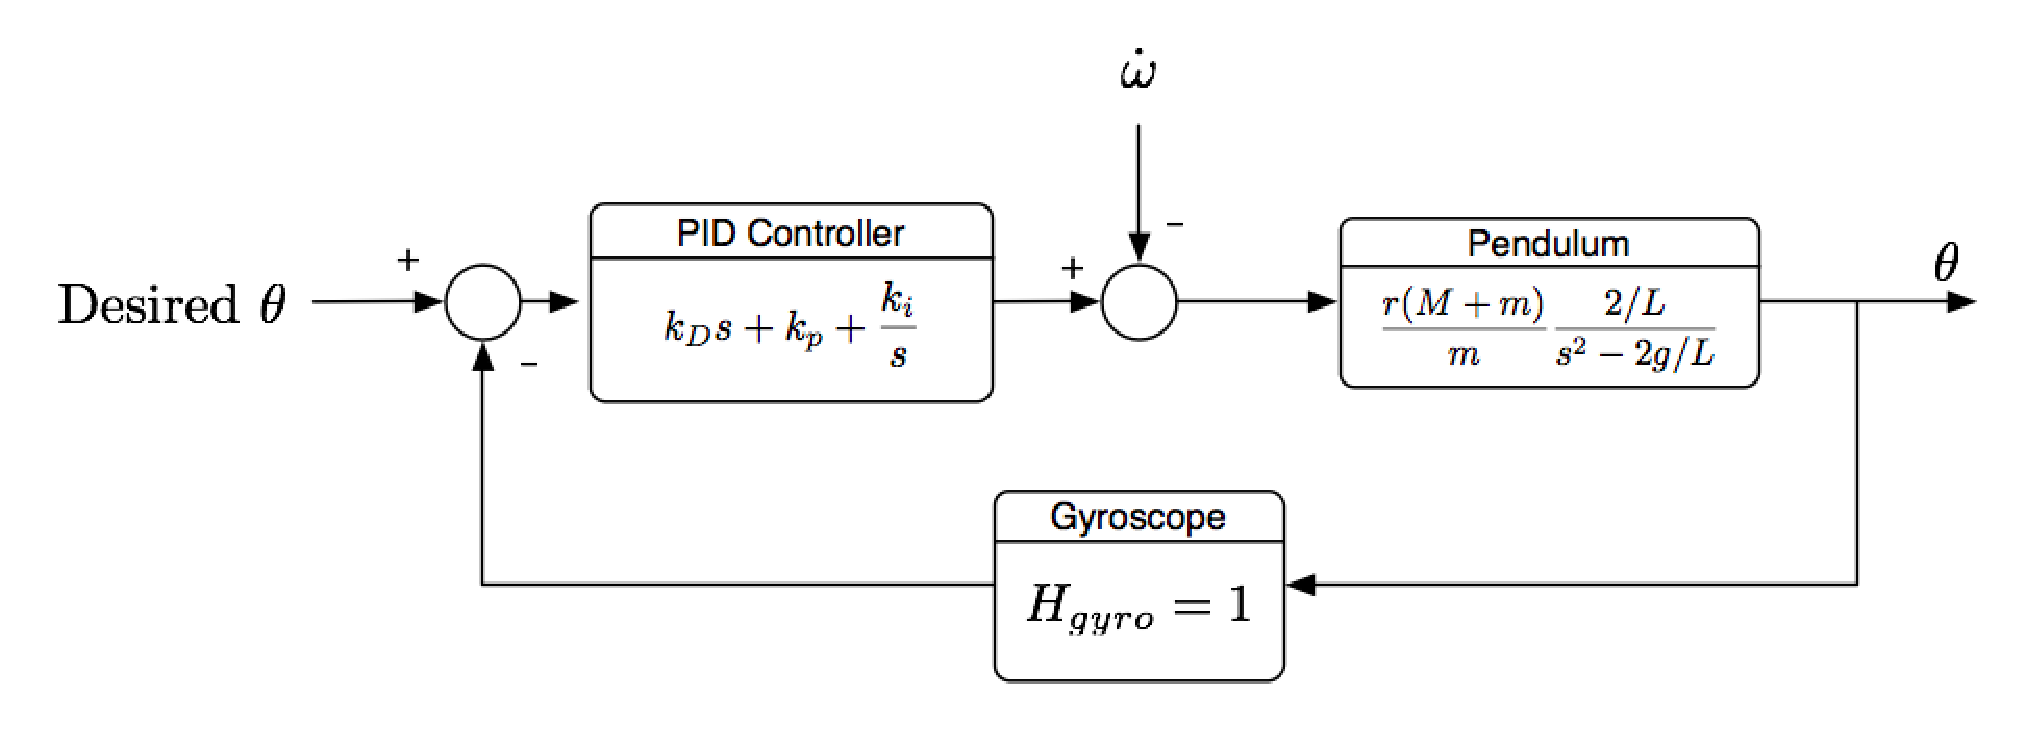
\includegraphics[width=5 in]{pics/Block_Diagram_2.eps}
  \end{center}
  \caption{Block diagram for our system}
  \label{fig:block_diagram}
\end{figure}

\begin{figure}[!h]
  \begin{center}
    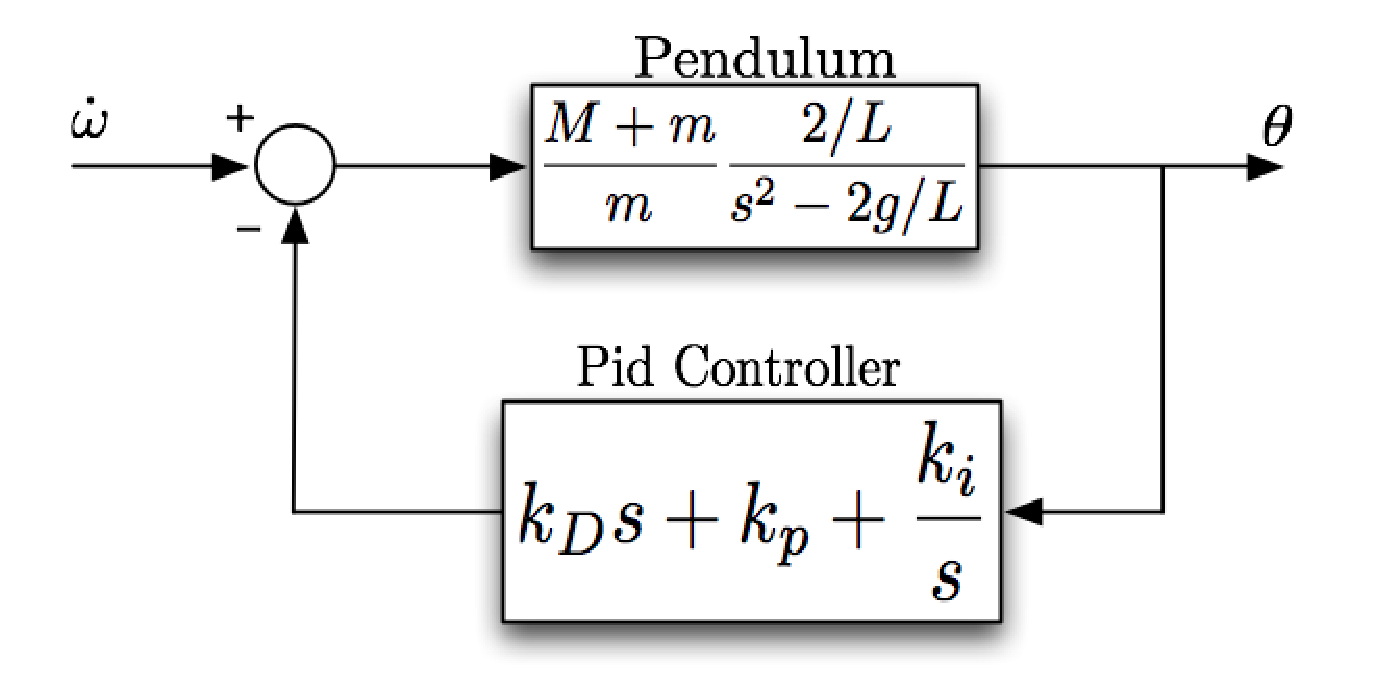
\includegraphics[width=4 in]{pics/Block_Diagram_3.eps}
  \end{center}
  \caption{Another way to understand  our system}
  \label{fig:block_diagram_3}
\end{figure}

We used Matlab to tune $K_p$, $K_D$, and $K_i$, giving them values of $K_D=20$, $K_p=300$, and $K_i=1$. We are estimating the friction coefficient to be about 0.8. This is tentative, however.

We can redraw this block diagram in the way shown on the next page. This is a different but equally valid  way of conceptualizing our system. In this system, the desired $\theta$ has been removed since it is equal to 0. The input to our system is now the disturbance acceleration, while  the PID controller is in the feedback loop. The gyroscope has been removed for additional simplification. 

\newpage
\section{Performance Measurements}
The full system was simulated in Matlab. The settling time was found to be 1.22 seconds and the bode plot met the performance specifications.

\begin{figure}[!h]
  \begin{center}
    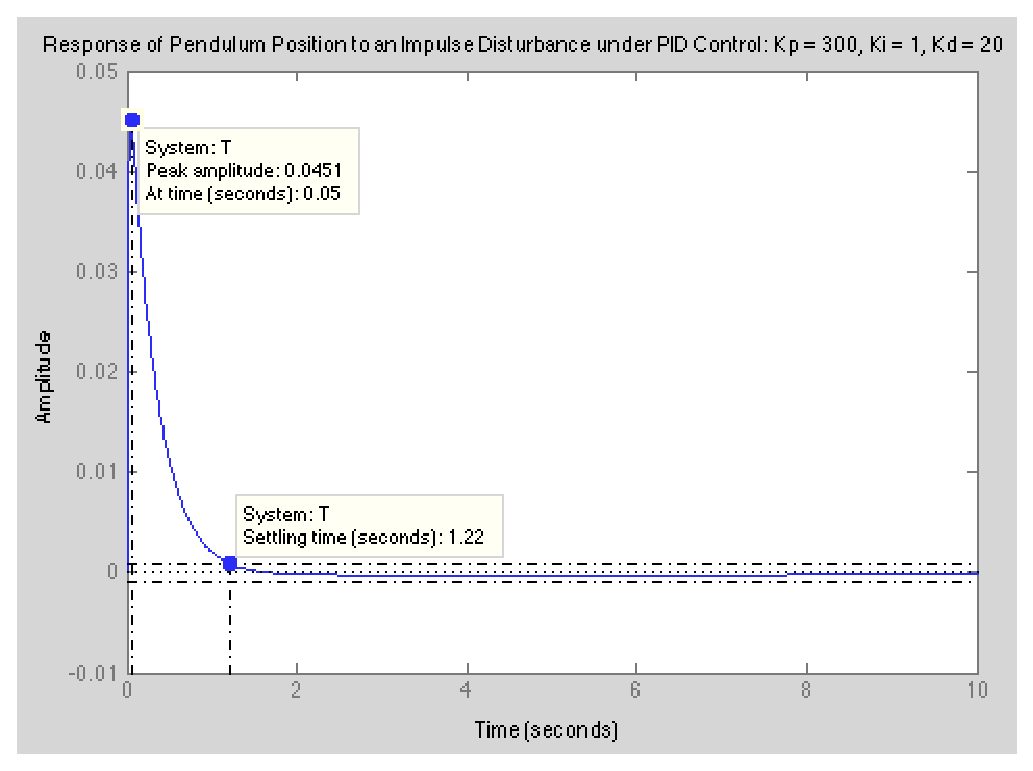
\includegraphics[width=5 in]{pics/performance_measurements/impulse_response_perf.eps}
  \end{center}
  \caption{Impulse response of our system}
  \label{fig:impulse_response}
\end{figure}

\begin{figure}[!h]
  \begin{center}
    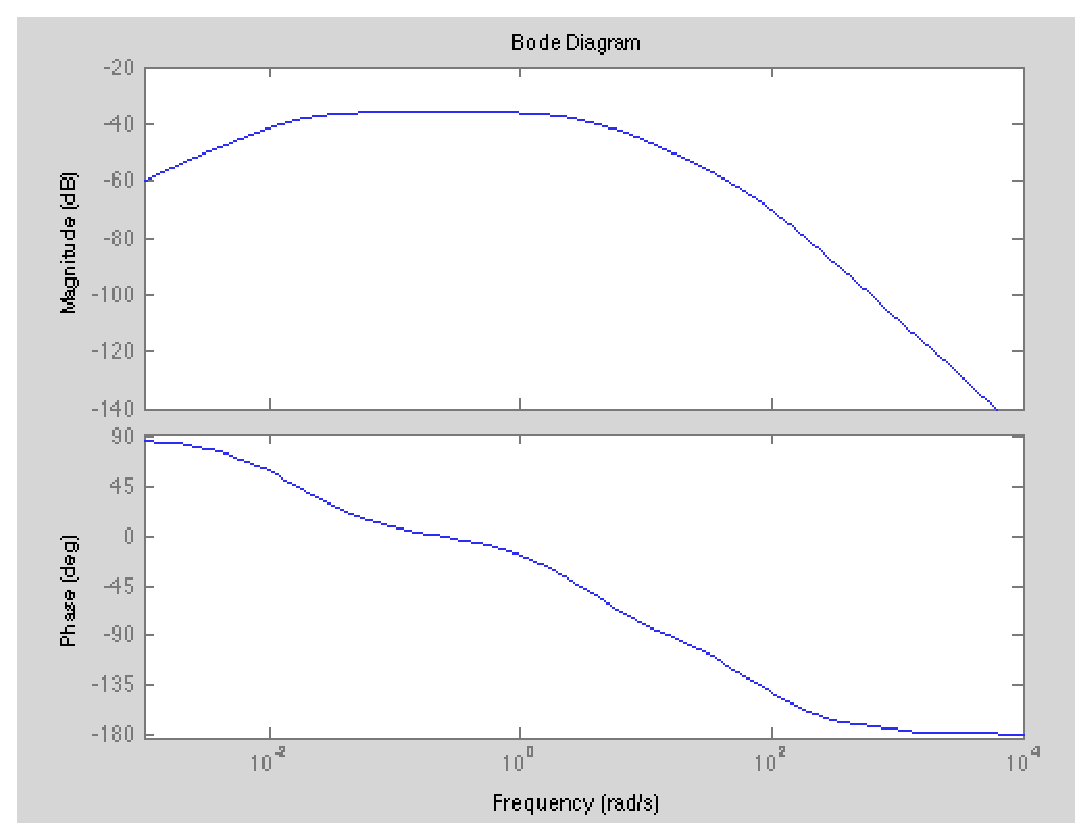
\includegraphics[width=5 in]{pics/performance_measurements/bode_plot.eps}
  \end{center}
  \caption{The Bode plot of our system.}
  \label{fig:bode_plot}
\end{figure}

Here is the Matlab code:
\MatLab{Matlab code for tuning}{lst:tuning}{../Matlab/PID_Design.m}
%\newcommand{\MatLab}[3]{
%  \lstset{language=Matlab}
%  \lstset{backgroundcolor=\color{listinggray},rulecolor=\color{blue}}
%  \lstset{linewidth=\textwidth}
%  \lstset{commentstyle=\textit, stringstyle=\upshape,showspaces=false}
%  \lstset{frame=tb}
%  \lstinputlisting[caption={Matlab code for tuning},label={matlab_code}]{~/Documents/Inverted_Pendulum/Matlab/PID_Design}





\end{document}
